\documentclass[12pt,a4paper]{article}
\usepackage[utf8]{inputenc}
\usepackage[german]{babel}
\usepackage{amssymb}
\usepackage{amsmath}
\usepackage{amsfonts}
\usepackage{tikz}
\usetikzlibrary{arrows ,automata ,positioning}
\usepackage{amssymb}
\usepackage{graphicx}
\usepackage{epstopdf}
\usepackage{tabto}
\usepackage[left=2cm,right=2cm,top=2cm,bottom=2cm]{geometry}
\usepackage{listings}
\lstset{
	language=bash,
	basicstyle=\ttfamily
}
\author{Christian Grieß}
\begin{document}
\begin{titlepage}
\begin{figure}
	\centering 
\includegraphics[scale=1]{HTW_LOGO.png}
\end{figure}

	
	\centering
	{\scshape\LARGE hochschule für Technik und Wirtschaft Dresden \par}
	\vspace{2cm}
	{\scshape\Large Übertragung von Sensordaten mittels LoRaWAN\par}
	\vspace{0cm}
	{\scshape\Large Projektseminar \par}
	\vspace{1.5cm}
	{\huge\bfseries Katastrophennetz\par}
	{\huge\bfseries mithilfe von Meshtastic\par}
	\vspace{1.5cm}
	{\huge\bfseries {Dokumentation}\par}	
	\vspace{4cm}
	{\Large\itshape Christian Grieß\par}
	{\Large\itshape Göran Heinemann\par}
	{\Large\itshape Julian Meinking\par}
	\vfill
	unter Aufsicht von\par %betreut von
	Prof. Dr.-Ing.~Jörg \textsc{Vogt}

	\vfill

% Bottom of the page
	{\large \today\par}
\end{titlepage}
\newpage
\tableofcontents

\newpage
\section{Aufgabenstellung}

Ziel dieses Projekts war das Experimentieren mit Meshtastic auf LoRa-fähigen Geräten.
Meshtastic ist ein Open-Source-Projekt, das es ermöglicht, ein Mesh-Netzwerk aufzubauen, das auf der LoRa-Technologie basiert. Es ist eine kostengünstige und energieeffiziente Möglichkeit, ein Netzwerk aufzubauen, das unabhängig von Internet und Mobilfunknetzen funktionieren kann.

\section{Fragestellung}

Ist Meshtastic als unabhängiges Kommunikations-Netzwerk für den Krisenfall im Raum Dresden geeignet?

\section{Technologie}
\subsection{Was ist LoRa?}

LoRa (von Long Range) ist eine proprietäre Funktechnologie im Besitz von Semtech. Sie ist für die Langstreckenübertragung (z.B. 10 km), schmalbandige Übertragung (gemessen in Kbps) und energiesparende Kommunikation konzipiert, hauptsächlich für Internet of Things (IoT)-Netzwerke. Dafür wird eine drahtlose Modulationstechnik, die aus der Chirp Spread Spectrum (CSS)-Technologie abgeleitet ist verwendet. Sie codiert Informationen auf Radiowellen mithilfe von Chirp-Impulsen! Die modulierte Übertragung von LoRa ist robust gegen Störungen und kann über große Entfernungen empfangen werden.

Es eignet sich ideal für Anwendungen, die kleine Datenmengen mit niedrigen Bitraten übertragen. Daten können über eine längere Reichweite übertragen werden im Vergleich zu Technologien wie Wlan, Bluetooth oder ZigBee. Diese Eigenschaften machen LoRa besonders geeignet für Sensoren und Aktoren, die im Niedrigenergiemodus arbeiten.

Außerdem arbeitet LoRa in einem lizenzfreien Sub-Gigahertz-Frequenzband (d.h. unter 1 GHz), aber die zu verwendenden Frequenzen variieren von Region zu Region aufgrund regulatorischer Anforderungen. Wenn Sie ein LoRa-Gerät kaufen, muss sichergestellt sein, dass das richtige Frequenzband unterstützt wird.

In Europa - 863–870MHz (normalerweise 868MHz).

\subsection{Warum LoRa?}

LoRa versucht die Lücke zwischen zwischen Kommunikationstechnologien wie WiFi, Bluetooth und LTE zu schließen.\\

\begin{figure}
	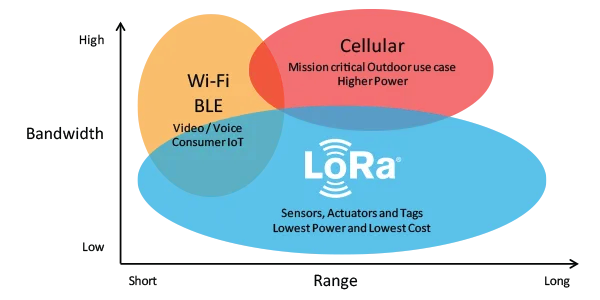
\includegraphics[scale=0.7]{bandwidth-vs-range.png}
\end{figure}
Semtech

Es ist für große Reichweite, kleine Bandbreite und Niedrigenergiekommunikation gemacht. Alles in allem also extrem nützlich für IoT Geräte. Einige Beispiele sind:

\begin{itemize}
	\item Wassersensoren in einer entfernten Umgebung (Grundwasser)
	\item Rauchwarnmelder
	\item Tierbeobachtung
	\item Verbrauchsmessungen bei Endkunden (Gas, Strom)
	\item Wetterstationen die nur ab und zu Informationen übertragen
\end{itemize}

\subsection{LoRa und LoRaWAN}

LoRaWAN ist über LoRa angesiedelt und definiert das Kommunikationsprotokoll und die Systemarchitektur.

Es ist wichtig zu verstehen, dass es möglich ist LoRa ohne LoRaWAN zu benutzen. Andere LoRa basierte Netzwerke sind Helium, The Things Network Disaster.radio und, was wir weiter betrachten werden, Meshtastic.

\subsection{Meshtastic}
Wie im vorherigen Absatz erwähnt, baut Meshtastic auf LoRa auf und schafft ein dezentralisiertes Mesh-Netzwerk.

Es bringt folgende Eigenschaften mit sich:
\begin{itemize}
	\item Verschlüsselte und Textbasierte Kommunikation
	\item Plattformunabhängig
	\begin{itemize}
		\item Computer (unabhänging vom Betriebssystem)
		\item Android (dedizierte Chat-App)
		\item iOS (dedizierte Chat-App)
	\end{itemize}
	\item Dezentralisiert
	\item Geringer Stromverbrauch
	\item Optionales Standort teilen
	\item Open-source
\end{itemize}

Anders als traditionelle Mobilfunknetzwerke, verbindet sich jedes Endnutzergerät mit einem LoRa Radio und alle LoRa Radios, welche Meshtastic nutzen, können Nachrichten, selbst wenn die Radios nicht im gleichen Mesh sind, weiterleiten. Das passiert so lange, bis die Nachricht Ihr Ziel erreicht oder die voreingestellten “Hops” ausgeschöpft werden.

\section{Geräte}

Folgende Geräte haben wir für das Projekt genutzt:

\subsection{Heltec LoRa32 v3}

https://heltec.org/project/wifi-lora-32-v3

max TX power: +21dBm

\begin{figure}
	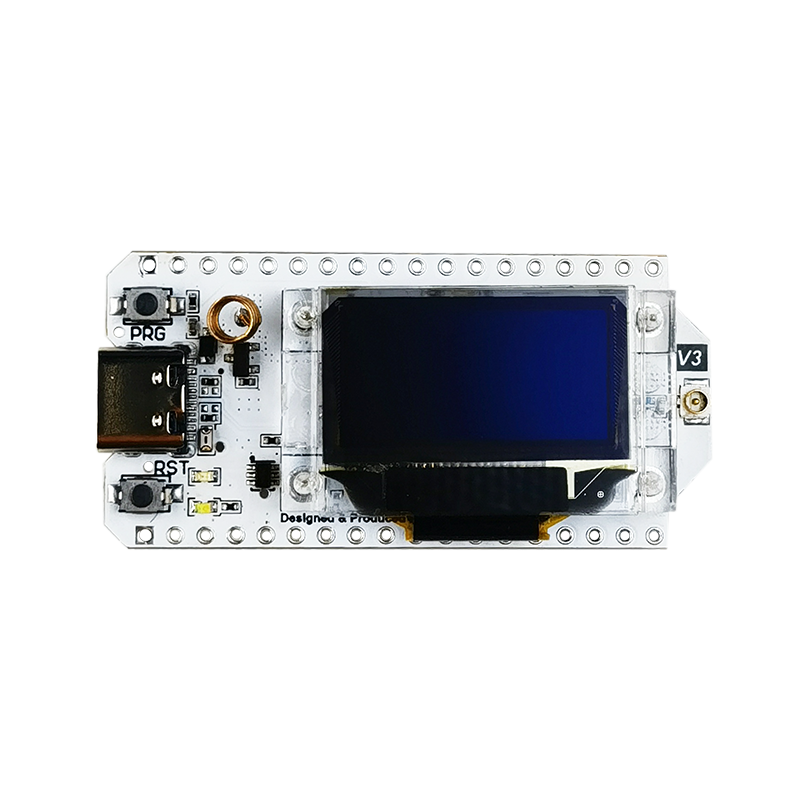
\includegraphics[scale=0.1]{heltec-lora32-v3.png}
\end{figure}

\subsection{LILYGO T-Echo}

https://www.lilygo.cc/products/t-echo


max TX power: +21dBm

\begin{figure}
	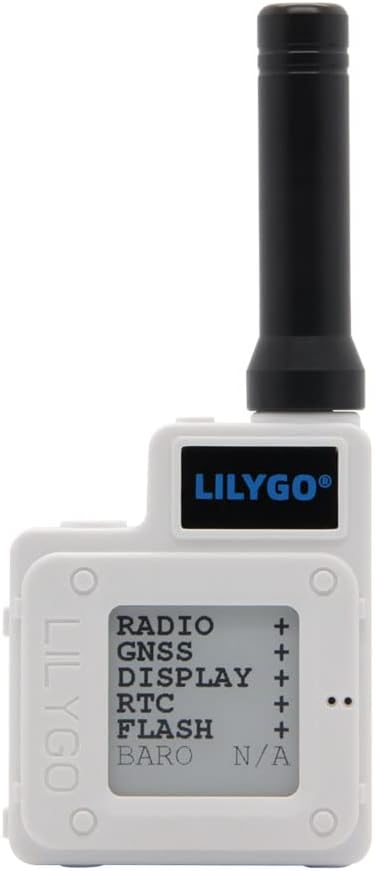
\includegraphics[scale=0.1]{t-echo.jpg}
\end{figure}

\subsection{LILYGO T-Deck}

https://www.lilygo.cc/products/t-deck


max TX power: +21dBm

\begin{figure}
	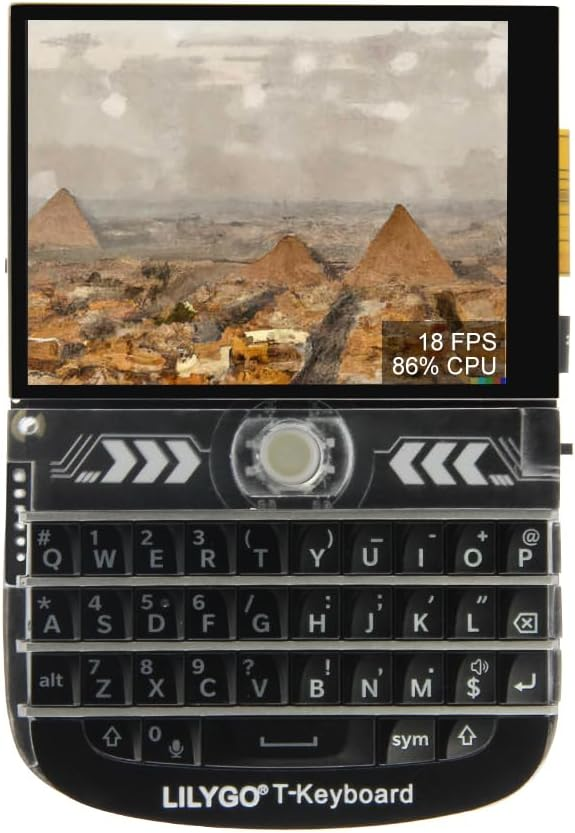
\includegraphics[scale=0.1]{t-deck.jpg}
\end{figure}

\section{Firmware flashen}
Geräte brauchen Firmware

\subsection{Hardware identifizieren oder auswählen}
Achtung!
Vorweg, Geräte nur mit angeschlossener Antenne einschalten! Anderenfalls kann das Gerät sich im schlimmsten Fall selber zerstören.

Meshtastic wird offiziell nur von bestimmten Geräten welche ein LoRa Modul innehaben supportet.

Es ist darauf zu achten, dass jedes Gerät welches im Meshnetz betrieben werden soll auf der gleichen Frequenz arbeitet. Hier gibt es unterschiede!

In deutschland können die freien Frequenzbänder 433 MHz und 868MHz, auf welchen Lora operiert, ohne Lizenzkosten oder Amateurfunklizenz genutzt werden.

Solange WLAN Verbindung zu einem Device nicht notw. ist und Bluetooth ausreicht, sollte ein nRF52 Chip gewählt werden, da diese energieffizienter als ESP32 Chips und einfacher zu flashen sind. Es gibt auch noch Geräte auf Basis des RP2040, diese haben wir allerdings nicht getestet.

Eine Liste mit unterstützer Hardware findet sich hier:

https://meshtastic.org/docs/hardware/devices/

\subsubsection{Serial Treiber für ESP32}
Einen für das eigene Betriebssystem passenden Treiber auf folgender Seite identifizieren, herunterladen und Installieren:

https://meshtastic.org/docs/getting-started/serial-drivers

\subsubsection{Serial Treiber für nRF52}
nRF52 Chips benötigen normalerweise keinen Serial Treiber. Sie benutzen einen UF2 bootloader, welche das Gerät als USB-Stick vom Betriebssystem erkennen lassen.

Auf keinen Fall folgenden USB geräte treiber herunterladen, es sei denn es wird UF2 support benötigt

https://meshtastic.org/docs/getting-started/serial-drivers/nrf52

\subsection{Firmware für ESP32 flashen}
https://meshtastic.org/docs/getting-started/flashing-firmware/esp32/ Da es bei uns auf verschieden PCs probleme gab haben wir zum Flashen unter Linux eine Nix-Flake erstellt, die Python mit den richtigen Paketen installiert und eine kleine Anleitung (auch zum selber Compilieren der Firmware) für esp32 und nRF52 Geräte enthät.

\subsection{Firmware für ESP32 nRF52}
https://meshtastic.org/docs/getting-started/flashing-firmware/nrf52/ Beim diesen Geräten ist es bei uns manchmal vorgekommen, dass das Flashen von Firmware zwar bis zu dem “Drag und Drop”-Schritt funktioniert und dann aber nicht wirklich mit der neuen Version neu startet. Falls das passiert muss man sich mit einer seriellen Konsole mit dem Gerät verbinden und einfach nur einmal Enter drücken, besonders nachdem Factory-Erase. Das steht unter dem Punkt Factory-Erase auch dokumentiert, aber man benötigt nicht zwingend die Meshtastic CLI, sondern lediglich ein Programm wie z. B. minicom unter Linux.

\section{Häufige Probleme - Kommunikation mit Gerät über USB}
\begin{itemize}
	\item Die Gerät-Datei /dev/ttyUSB0 gehört der Nutzergruppe dialout. Damit der Nutzer Schreibrechte erhalten kann, muss er zur Gruppe hinzugefügt werden:
	
	\lstinline{sudo usermod -aG dialout <user-name>}
	
	Der Nutzer muss sich ausloggen und wieder einloggen, damit er in der Gruppe enthalten ist.
	\item Prüfen, ob das Kabel zwischen Computer und Gerät auch wirklich Daten übertragen kann.
	\item USB-C → USB-C funktioniert manchmal nicht. Dies könnte an einem Fehler bei USB-C Power Delivery liegen. Adapter USB-C → USB-A (findet man meist als OTG-Adapter) schafft Abhilfe.
\end{itemize}

\section{Werkzeuge}
\begin{description}


    \item [Programmiersprache]\tab Python
    \item [Open-Source Bibliotheken]\tab Keras \newline \tab \tab Tensorflow
 
 
\end{description}

\section{Was ist Maschinelles Lernen?}
Maschinelles Lernen ist das Fachgebiet, das Computern die Fähigkeit zu lernen verleiht ohne explizit programmiert zu werden
\begin{flushright} - Arthur Samuel 1959  \end{flushright}

\section{Was sind Rekurrente Neurale Netzwerke?}
Placeholder

\subsection{ML-Modell}
$<Grafik>$ \newline
Placeholder
\subsubsection{GRU-Layer}
Why GRU (Vorteile, Nachteile) \newline
Verallgemeinerte(vereinfachte) Grafik (Update Gate, Reset Gate, Current Memory)\newline
Grafik Update Gate\newline
etc.
\subsubsection{LSMT-Layer}
Placeholder
\subsubsection{Dense-Layer}
Placeholder
\subsubsection{Embedding-Layer}
Placeholder
\section{Codevorstellung und Beschreibung$(Einzelschritte?)$}
Placeholder incl. Auswertungsgrafiken
\newpage

\section{Discussion}
\section{Summary}
\section{References}
\end{document}
